\documentclass[11pt,handout]{beamer}
\mode<article> % only for the article version
{
  \usepackage{fullpage}
  \usepackage{hyperref}
%\usepackage[ps2pdf]{hyperref}
}
\usepackage{epsfig}
\usepackage{fancybox}

\mode<presentation>
{
%  \setbeamertemplate{background canvas}[vertical shading][bottom=white,top=blue!10]
%     \usetheme{Warsaw}
% \usetheme{CambridgeUS}
%  	\usetheme{Frankfurt}
%  	\usetheme{Berlin}
%  	\usetheme{Antibes}
%   \usetheme{Darmstadt}
%    \usetheme{Madrid}
%    \usefonttheme[onlysmall]{structurebold}
 	\usecolortheme{orchid}
% 	\usecolortheme{seahorse}
  \usecolortheme[named=blue]{structure}
% 	\usecolortheme{crane}
%	\usecolortheme{lily}
}

\setbeamercolor{math text}{fg=green!50!black}
\setbeamercolor{normal text in math text}{parent=math text}

\usepackage{epsfig}
\usepackage{amsmath}
\usepackage{amssymb}
%\usepackage{beamerthemesplit}
\usepackage{listings}
\usepackage[vlined,algoruled,titlenotnumbered,linesnumbered]{algorithm2e}


%\usepackage{lmodern}
%\usepackage[T1]{fontenc} 

\usepackage{times}

\setbeamercovered{dynamic}

\title[NLP]{Natural Language Processing}
\subtitle{Lecture I. Introduction and Syllabus}
\author[Forrest Sheng Bao]{Forrest Sheng Bao, Ph.D.}
\institute[ISU]{Dept. of Computer Science \\ Iowa State University \\ Ames, IA 50011}
\date[8/23/2022]{Aug. 23, 2022}

%\AtBeginSection[] {
%  \begin{frame}[plain]
%    \frametitle{Outline}
%    \tableofcontents[currentsection]
%  \end{frame}
%  \addtocounter{framenumber}{-1}
%}

\AtBeginSubsection[] {
  \begin{frame}[plain]
   \frametitle{Outline}
    \tableofcontents[currentsubsection]
    \addtocounter{framenumber}{-1}
  \end{frame}
} 

\begin{document}

 \frame{\titlepage}
 
 \section<presentation>*{Outline}
 
   \begin{frame}
     \frametitle{Outline}
  \tableofcontents
   \end{frame}

\section{The Instructor}

% \begin{frame}{The Instructor}
% \begin{block}{Background}
%  \begin{itemize}
%   \item Undergraduate: EE
%   \item No MS degree. 
%   \item PhD: CS
%   \item Postdoc: neuroscience at medical school
%   \item Past 4 years: A EE professor
%   \item Now: A CS professor
%   \item My PhD thesis is not on NLP but on KR and planning. 
%  \end{itemize}
% \end{block}
% \end{frame}

\begin{frame}{The Instructor}
% \begin{block}{Not a typical Asian student/professor}
%   \begin{itemize}
%    \item suspended twice in high school - extremely undisciplined 
%    \item college GPA under 3.0 but made to grad school (inspired by a GaTech EE professor who also had a sub3.0 GPA and thanks to my PhD advisor)
%    \item horrible test scores before grad school
%    \item I just like to figure out things very much. 
%   \end{itemize}
% \end{block}
% 
% \pause

\begin{block}{My research}

My PhD dissertation is not on NLP, ML nor CV. My PhD dissertation is about GOFAI. 

\pause 

\begin{itemize}
 \item Artificial Intelligence 
 \begin{itemize}
  \item Knowledge Representation and Reasoning
  \item Natural Language Processing
 \end{itemize}
 \item AI's applications in other sciences
 \begin{itemize}
  \item Routing and palcements in IC and PCB designs
  \item Reinforcement learning for storage systems 
  \item NLP for biomedical papers
 \end{itemize}
\end{itemize} 
\end{block}

\pause

\begin{block}{Carl Gauss, Letter to Bolyai (1808)}
\textit{When I have clarified and exhausted a subject,  \\
then I turn away from it,  \\
in order to go into darkness again.} 
\end{block}

 \pause

* I am a tenth generation academic descendant of Carl Gauss. 

\end{frame}

\section{Natural Language Processing}

\begin{frame}{What (Un)Natural Languages are}

\hskip -2em
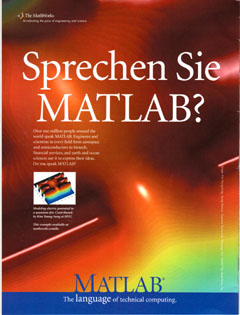
\includegraphics[width=0.35\textwidth]{figures/matlab_de.jpg} 
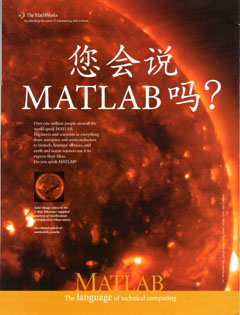
\includegraphics[width=0.35\textwidth]{figures/matlab_zh.jpg} 
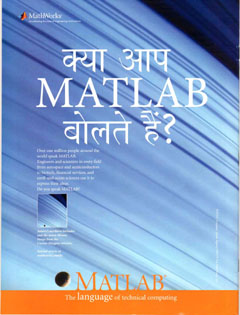
\includegraphics[width=0.35\textwidth]{figures/matlab_hi.jpg}

 \begin{itemize}[<+->]
  \item Lots of data, e.g., Amazon reviews 
  \item Against computer programming languages 
  \item Very easy to handle: discretized objects
  \item Very difficult to handle: unstructured, ambiguity, variety, etc. 
 \end{itemize}
\end{frame}

\begin{frame}{Why do we study NLP...instead of other hot areas in AI}
 \begin{itemize}
  \item Unlike other animals, we have complicated langauges. \pause
  \item Languages make us great\pause: 
  \small{
    \begin{exampleblock}{}
   ``a group of people get together and exist as an institution that we call a company so they are able to accomplish something collectively which they could not accomplish separately''\pause -- The HP Way.  
    \end{exampleblock}
    }
  
  \item When we spoke the same langauge, even God was afraid. 
  
  \begin{exampleblock}{}
   `` And the LORD said, Behold, the people is one, and they have all one language; and this they begin to do: and now nothing will be restrained from them, which they have imagined to do.''  --Genesis 1:6
  \end{exampleblock}
  
  \item NLP is about understanding ourselves. 
%   \item ``The problem of neurology is to understand human himself.''
%   \item The problem of NLP is to understand human himself in a latent or blackbox way.
 \end{itemize}
\end{frame}

\begin{frame}{NLP vs. speech-related research}
  \begin{itemize}
    \item NLP usually does not cover speech-related research, such as automatic speech recognition (ASR, speech-to-text) or speech synthesis (text-to-speech, TTS)
    \item Speech is about vocal time series, acoustic signals, or waves.
    \item NLP usually deals with the written form of languages, i.e., the scripts. 
    \item For example, Siri, Cortana, Alexa have both speech part and NLP part. 
  \end{itemize}
\end{frame}


\begin{frame}{NLP is far from expectation (circa. 2018)}
 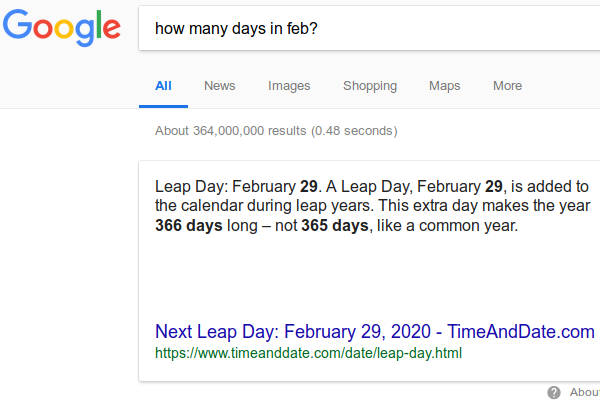
\includegraphics[width=\textwidth]{figures/how_many_days_in_feb.png} 
\end{frame}

\begin{frame}{NLP is far from expectation (circa. 2018)}
 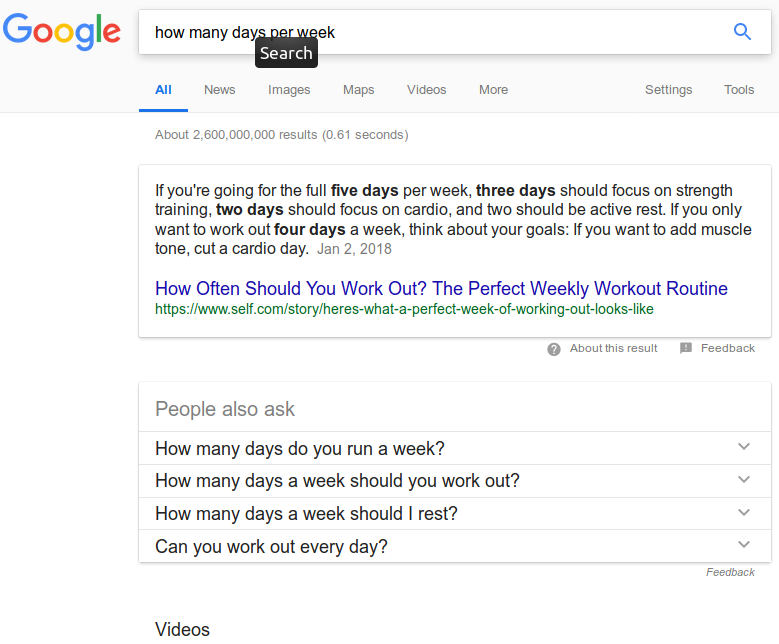
\includegraphics[width=\textwidth]{figures/how_many_days_per_week.png} 
\end{frame}

\begin{frame}{Winograd Schema Challenge (WCS)}
\begin{exampleblock}{Let's fill a blank}
 The city councilmen refused the demonstrators a permit because they [~~~~~~~~~~~~~~~]  violence.
 
 A. feared 
 
 B. advocated
\end{exampleblock}

 
\end{frame}


\begin{frame}{NLP is far from expectation}
Spell checking is NLP. 

 
\includegraphics[width=\textwidth]{figures/Microsoft_spellchecker_I_hir_waiting_for_you.png} 
\end{frame}

\begin{frame}{NLP is far from expectation (circa. 2018)}
Spell checking is NLP. 

 
\includegraphics[width=\textwidth]{figures/Microsoft_spellchecker_I_will_all_you_in_5_minutes.png} 
\end{frame}

\begin{frame}{NLP in AI}
 \begin{itemize}[<+->]
\item Alan Turing 1950 paper   ``Computing Machinery and Intelligence''
\item Early sci-fi movies all have what today we call ``question answering'' (QA) or ``automatic speech recognition'' (ASR): Startrek communicator, 2001: A Space Odyssey (HAL can even read our lips! )
\item Machine translation as at the center of early AI research 
\item ``the spirit is willing but the flesh is weak'' $->$ Russian and back $->$ ``the vodka is good but the meat is rotten.''
\item Almost no AI funding by 1974 -- first AI winter.     
\item Reading assignment: ``Technology; The Computer As Translator'', New York Times, April 28, 1983. \url{https://www.nytimes.com/1983/04/28/business/technology-the-computer-as-translator.html}
\end{itemize}
\end{frame}

\begin{frame}{American academia should stop chasing buzzwords and imminent applications}
 \begin{itemize}[<+->]  
   \item Almost half a century later, after two AI winters, machine translation final becomes plausible. 
   \item Automatic speech recognition (ASR) also comes into our daily life: Google Now, Amazon Alexa, Apple Siri, Microsoft Cortana, etc. 
   \item Persistent research into neural networks (or in today's buzzword, ``deep learning'') made those task tractable. 
   \item Ironically, ``neural network'' was almost dead in the US between mid 1990s and mid 2000s. Little funding. Few papers. Everyone was going after SVM.
   \item Hence, the deep learning wave started from Canada: Hinton (Toronto) and Y. Bengio (Montreal).
   \item Yann LeCun said in one of his Facebook posts that he was nobody until DL became popular. 
\end{itemize}
\end{frame}

\begin{frame}{Why NLP is hard}
\begin{itemize}[<+->]
 \item Ambiguity 1: \begin{itemize}
                   \item ``This book is mine.''
                   \item ``I live next to the coal mine.''
                   \item ``Millions of mines along the border is a result of the war.''
                  \end{itemize}
 \item Ambiguity 2: \begin{itemize}
                   \item ``You are so sweet.''
                   \item ``The soup is too sweet.''
                   \item ``Sweet, let's play the game!''
                  \end{itemize}
 \item Morphology 
 \begin{itemize}
  \item ``Carbon dioxide'' vs. CO$_2$
  \item ``Iowa State University'' vs. ``ISU''
  \item ``Step 1'' vs. ``First step'' 
 \end{itemize}
 \item We are not aware that we know so much. 
 \begin{itemize}
  \item This guy has two legs.  -- is it informative?
 \end{itemize}
\end{itemize}
\end{frame}


\begin{frame}{Typical tasks in or closely related to NLP (not mutually exclusive)}

%Just take a look at AC tracks. 

\begin{itemize}[<+->]
\item Spell checking, next-work prediction
\item Parsing and syntax
\item Named entity recognition (NER)
\item Relation/knowledge/information extraction, knowledge base/graph, e.g., \href{https://github.com/harperco/MeasEval}{MeasEval}
\item Information retrieval (historically considered a separate topic), e.g., Google search
\item Semantics (you may count word embedding into this)
\item Text classification  (e.g., was this review helpful?)
\item Machine translation
\item Automatic summarization (abstractive and extractive)
\item Question answering (QA)
\item Machine Reading Comprehension (MRC)
\item Text generation (a way to achieve many tasks aboves)
\item Sentiment analysis 
\item Topic modeling
\end{itemize}
\end{frame}


\begin{frame}[fragile]{Rule-based vs. statistical NLP}
 \begin{itemize}[<+->]
  \item There are general two approaches to NLP problems: Rule-based (expert system) vs. statistical (machine learning). 
  \item Tokenization is a typical task that rules may work without any problem. 
% \lstset{language=Python,
%                 basicstyle=\ttfamily,
%                 keywordstyle=\color{blue}\ttfamily,
%                 stringstyle=\color{red}\ttfamily,
%                 commentstyle=\color{green}\ttfamily,
%                 morecomment=[l][\color{magenta}]{\#}
% }
{\scriptsize
 \begin{verbatim}
>>> text = 'That U.S.A. poster-print costs $12.40...'
>>> pattern = r'''(?x)    # set flag to allow verbose regexps
...     ([A-Z]\.)+        # abbreviations, e.g. U.S.A.
...   | \w+(-\w+)*        # words with optional internal hyphens
...   | \$?\d+(\.\d+)?%?  # currency and percentages, e.g. $12.40, 82%
...   | \.\.\.            # ellipsis
...   | [][.,;"'?():-_`]  # these are separate tokens; includes ], [
... '''
>>> nltk.regexp_tokenize(text, pattern)
['That', 'U.S.A.', 'poster-print', 'costs', '$12.40', '...']
\end{verbatim}
}

\item However, there are many cases that rules cannot cover varieties. 
\item There shouldn't be a clear distinction between the two approaches. For example, is BOW model rule-based or statistical? 
 \end{itemize}
\end{frame}

\begin{frame}{KR needed in ML for NLP}
 
 Pure statistical language model is insufficient to judge whether the following statements makes a review helpful. 
  \begin{itemize} [<+->]
  \item ``a waste of money''
  \item ``Amazon shipping and return is so easy ''  
  \item  ``This car has 4 wheels '' 
 \end{itemize} 
\end{frame}

\begin{frame}{NLP is language-dependent}
 \begin{itemize}[<+->]
  \item Some tasks are particularly difficult in some languages, e.g., \href{https://nlp.stanford.edu/software/segmenter.shtml}{segmentation in Chinese and Arabic}. 
  \item Some tasks are not ``symmetric'' between languages, e.g., in machine translation, 
  \begin{itemize}
   \item a sentence in Chinese may be required by grammar to be broken into multiple sentences in English, or 
   \item the order of phrases needs to be rearranged after translation. 
  \end{itemize}
 \end{itemize}
\end{frame}

\begin{frame}{Computational Linguistics or NLP? }
\begin{itemize}
\item Apparently, mission-oriented research will not produce a long-lasting impact and/or a big breakthrough. 
\item ``Physics is like sex.'' Richard Feynman. 
\item  However, many problems in linguistics are not well defined, such as writing style. No ground truth. Hard to quantitatively measure. 
\item ``To create an artificial being has been the dream of man since the birth of science.'' 
\item Computer science is about processing information, maybe for human use. 
\item Hence, the instructor prefer the name NLP over CL. 
\end{itemize}

\end{frame}

\begin{frame}{What I am working on in NLP}
\begin{itemize}[<+->]
\item Review analysis  (``was this review helpful?'', ACL 2015, ICTAI 2016, EACL 2017, NAACL 2018, CIKM 2019)
\item Summarization (EACL 2017, and on going)
\item Summarization metrics (NAACL 2022, COLING 2022, and on going)
\end{itemize}
\end{frame}

\begin{frame}{About the class}
  \begin{itemize}
   \item Introductory: letting you know something about a lot of topics in NLP.
   \item NLP is so rapidly evolving so papers or online materials will be the main source of knowledge. 
   \item Project meeting with the TA/instructor once a week.  
  \end{itemize}
 \end{frame}

\begin{frame}{Outline of the class}
Let's go over the syllabus. 
\end{frame}

\begin{frame}{Prerequisite}
\begin{itemize}
\item Linear algebra, calculus (up to multivariate calculus or calculus III), Probability theory -- in era of deep learning, it is very hard to avoid such math basics.
\item Machine Learning -- however, we will spend some time to cover due to different background of students. 
\item Computer programming, e.g., you can solve Leetcode easy-level problems under 10 minutes. 
\item The patience and desire to to think systematically and structurally 
\end{itemize}
\end{frame}


% \begin{frame}{Example projects}
%  \begin{itemize}
%   \item Detecting events that are correlated, e.g., U. Akron esports. 
%   \item Personalized summary 
%   \item Summary based on knowledge increment 
%   \item Emoji recommendation based on CV
%   \item Purpose/discourse detection with context 
%   \item Natural way to define regexp, e.g., \url{https://github.com/BambooL/Natural-Expression}
%   \item Mining answers of questions from reviews. 
%   \item Finding explanations from multi-modal data. 
%   \item Just-in-time embedding 
%   \item Small enough language models, e.g., for emoji recommondation. 
%   \item Debiasing with common sense reasoning 
%   \item Pheonetic spell checking
%  \end{itemize}
% \end{frame}


% \begin{frame}{Homework 1}
% \begin{itemize}
% \item Read Alan Turing's 1950 paper ``Computing Machinery and Intelligence'', \url{http://phil415.pbworks.com/f/TuringComputing.pdf}
% \item Watch Kai-Fu Lee's 1993 presentation of ASR: \url{https://www.youtube.com/watch?v=PJ_KCTsOCrs} And write down your thoughts on how NLP can help ASR. 
% \item Read article ``The growing importance of Natural Language Processing'' from Wired \url{}https://www.wired.com/insights/2014/02/growing-importance-natural-language-processing/.
% \end{itemize}
% \end{frame}


\end{document}
